\documentclass{jhps}
\usepackage{amssymb}
\usepackage{mathtools}
\usepackage{booktabs}
\usepackage{multirow}
\usepackage{adjustbox}
\usepackage{footnote}
\usepackage{framed}
\usepackage{textcomp}
%\usepackage{verbatim}
\usepackage{adjustbox}
\usepackage{enumitem}
\usepackage{pmboxdraw} % to use UTF-8 inside a verbatim/listing environment
 % may use if needed
 %\usepackage{float}
 %\usepackage{array}
 %\usepackage{longtable}
 %\usepackage{comment}
 %\usepackage{pdflscape}
 %\usepackage{adjustbox}
 %\usepackage{tabularx}

\graphicspath{
{./assets/}
}

\begin{document}

\JHPSissue{0}   % keep 0 until the issue is assigned
\JHPSkeywords{Compression, NetCDF}   % add 2-5 keywords

  % Author macro takes Name, Institution, Optional Link to the person, Optional Email
\JHPSauthor{Max Müller}{My institution\\Berlin, Germany}{https://myinstitution.com/max}{max@müller.com}
\JHPSauthor{Priya Singh}{Another affiliation\\Bangladesh, India}{}{}   % use empty email here

\title{My Title}

  % add the section numbers to the listings/figures/tables
\counterwithin{lstlisting}{section}
\counterwithin{figure}{section}
\counterwithin{table}{section}

\maketitle

\begin{abstract}
This document provides a guideline to prepare the LaTeX document for the submission to JHPS.
Please check its source code to understand the proper usage of the formatting elements.

If the \verb|\JHPSissue| is set to $>0$, the header will slightly change.
The date of the document is the day the document was built.
\end{abstract}

\section{Introduction}
\label{sec:intro}

This document describes the formatting for JHPS.
Please check the LaTeX source code.
In \Cref{sec:intro}, the formatting style for different elements is described.

\subsection{Structure}

Use section, subsection, subsubsection, and paragraph.
A paragraph should introduce a new thought that is connected to the text.
For instance, as we use it here:

\paragraph{Justification} any other level of structure adds too much nesting to comprehend for the reader.

\subsection{Formatting}
You should use the font styles for the following purposes:
\begin{itemize}
  \item \textbf{bold} style to give list elements a name or when you define a term.
  \item \textit{italic} style to emphasize the use of specific terms or a subsentence.
\end{itemize}
You should not underline text.

\medskip

Generally use the given default font size, you may use small and scriptsize for bigger listings or verbatim environments but should not use it otherwise.

\medskip

Don't use \verb|\vspace| or \verb|\hspace| commands to adjust the placement of the objects.
You may use \verb|\bigskip| and \verb|\medskip| between paragraphs that are loosely connected.

\subsection{Floating elements}
Tables, figures, and listings are floating elements that can be placed on top, bottom, or extra places.
They need to provide a caption and label and must be referenced using cleveref, e.g., \verb|\Cref{tbl:name}|.
A caption should not end with a ".", except if it is a valid English sentence.

\subsubsection{Tables}
  %\usepackage{tabu}
  %\taburulecolor{EsiOrange}

For tables with a header, please use the formatting in \Cref{tbl:1a}.
Provide the unit in a secondary row.
Tables without a header can use a closed box as in \Cref{tbl:1b}.

\begin{table}
  \centering
  \begin{subtable}[t]{8cm}
  \centering
  \begin{tabular}{l|l|l}
         \rowcolor{tblhead} Experiment  & Throughput & Total perf.
  \\
         \rowcolor{tblhead}   & in IOPS & in MiB/s \\
       \hline
       \hline
   Config 1 & 1   &  2   \\
  \hline
   Config 2 & 4   &  5   \\
  \end{tabular}
  \caption{Caption 1}\label{tbl:1a}
  \end{subtable}
  %%%
  \begin{subtable}[t]{3cm}
  \centering
  \begin{tabular}{|l|l|l|}
  \hline
   1   &  2   &  3  \\
  \hline
   4   &  5   &  6  \\
  \hline
  \end{tabular}
  \caption{Caption 2}\label{tbl:1b}
  \end{subtable}
  \caption{Main table caption}\label{tbl:1}
\end{table}

\subsubsection{Figures}

\begin{figure}   % don't change placement [bpt] if possible
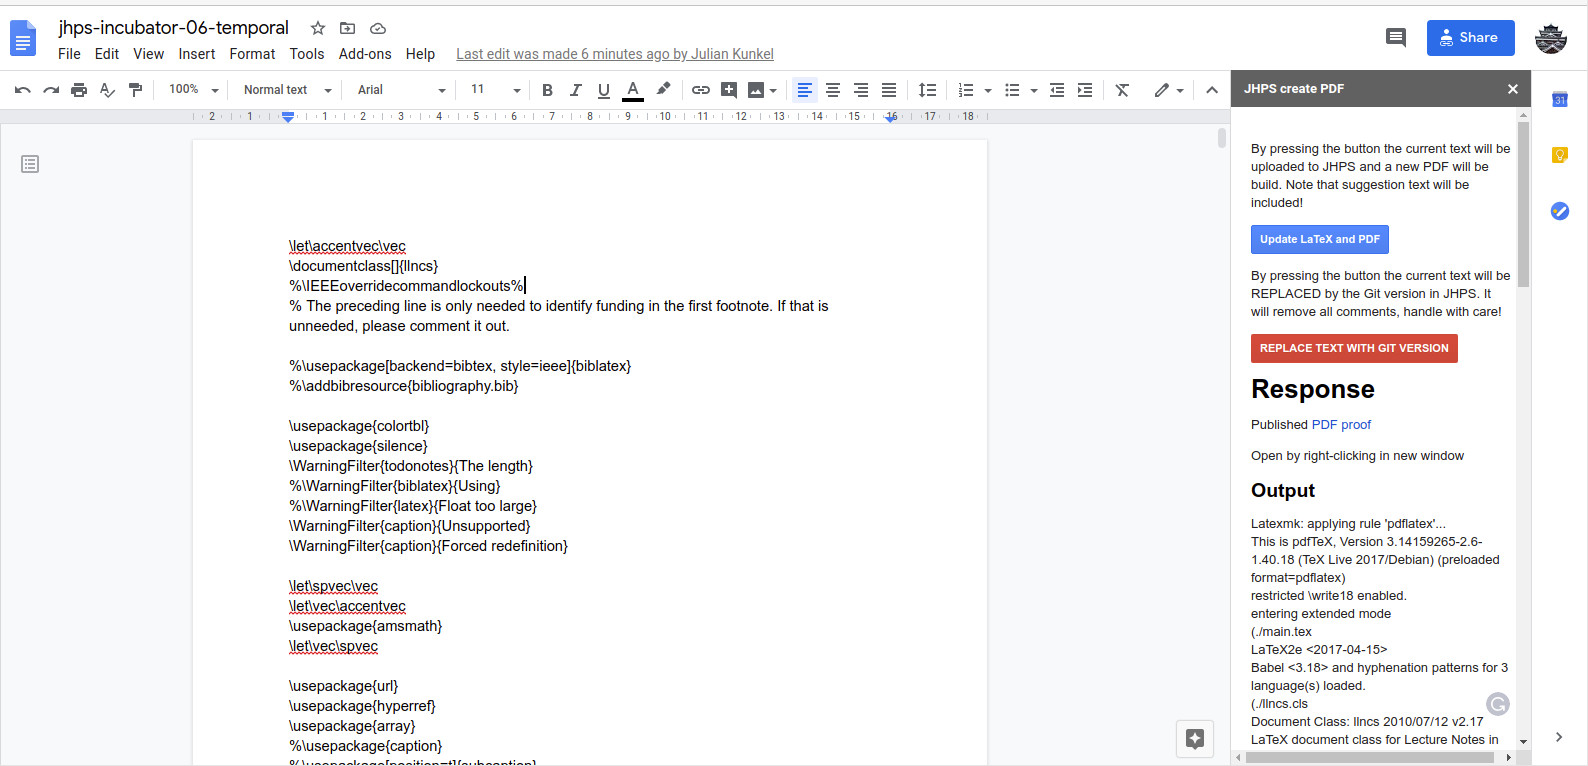
\includegraphics[width=0.8\textwidth]{jhps}
\caption{JHPS figure}
\label{fig:jhps}
\end{figure}

See \Cref{fig:jhps} for a simple figure.

\begin{figure}
  \begin{subfigure}[t]{3cm}
  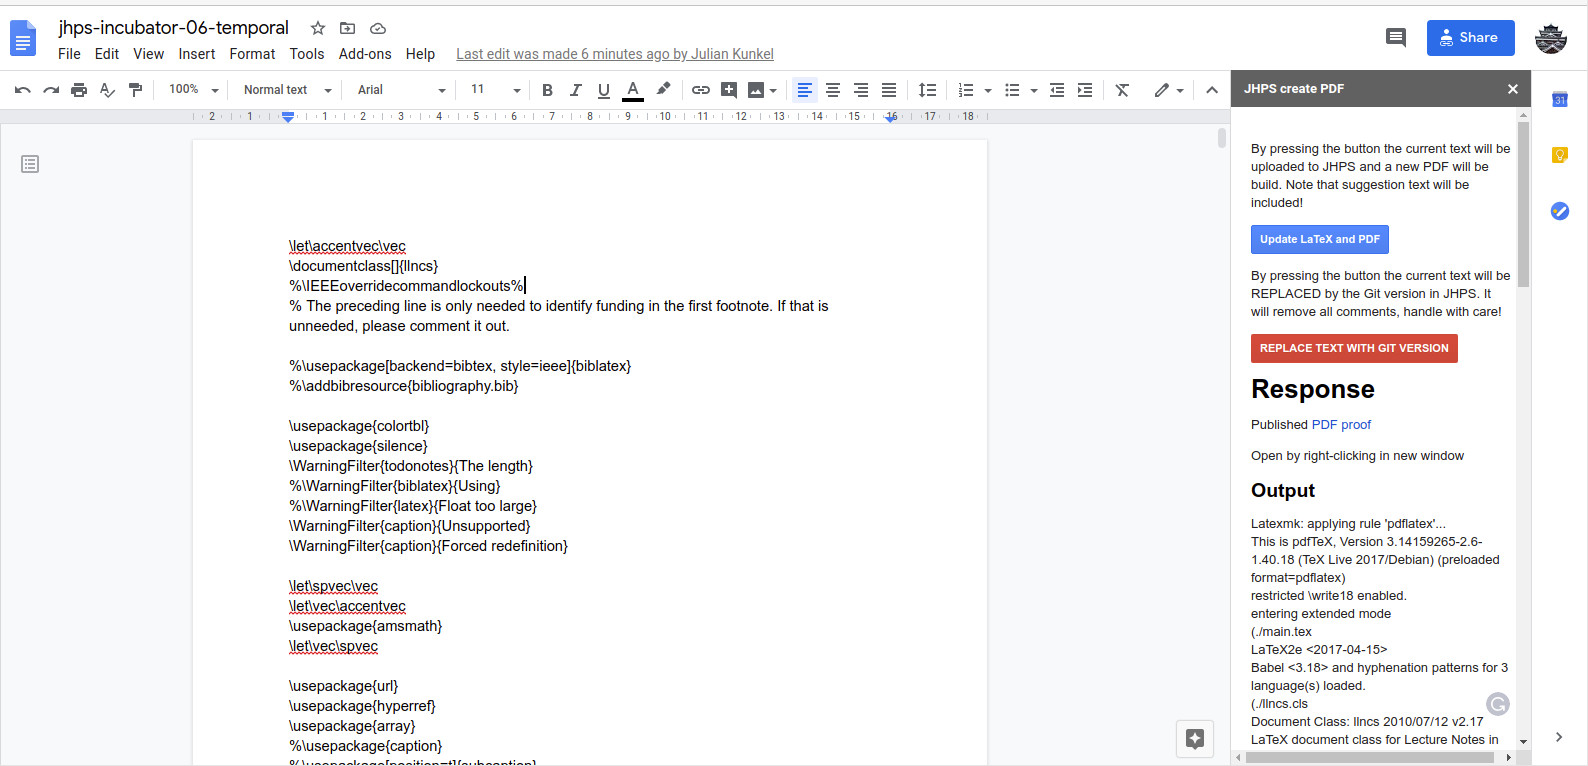
\includegraphics[width=\textwidth]{jhps}
  \caption{Caption 1}\label{fig:1a}
  \end{subfigure}
  \quad
  \begin{subfigure}[t]{3cm}
  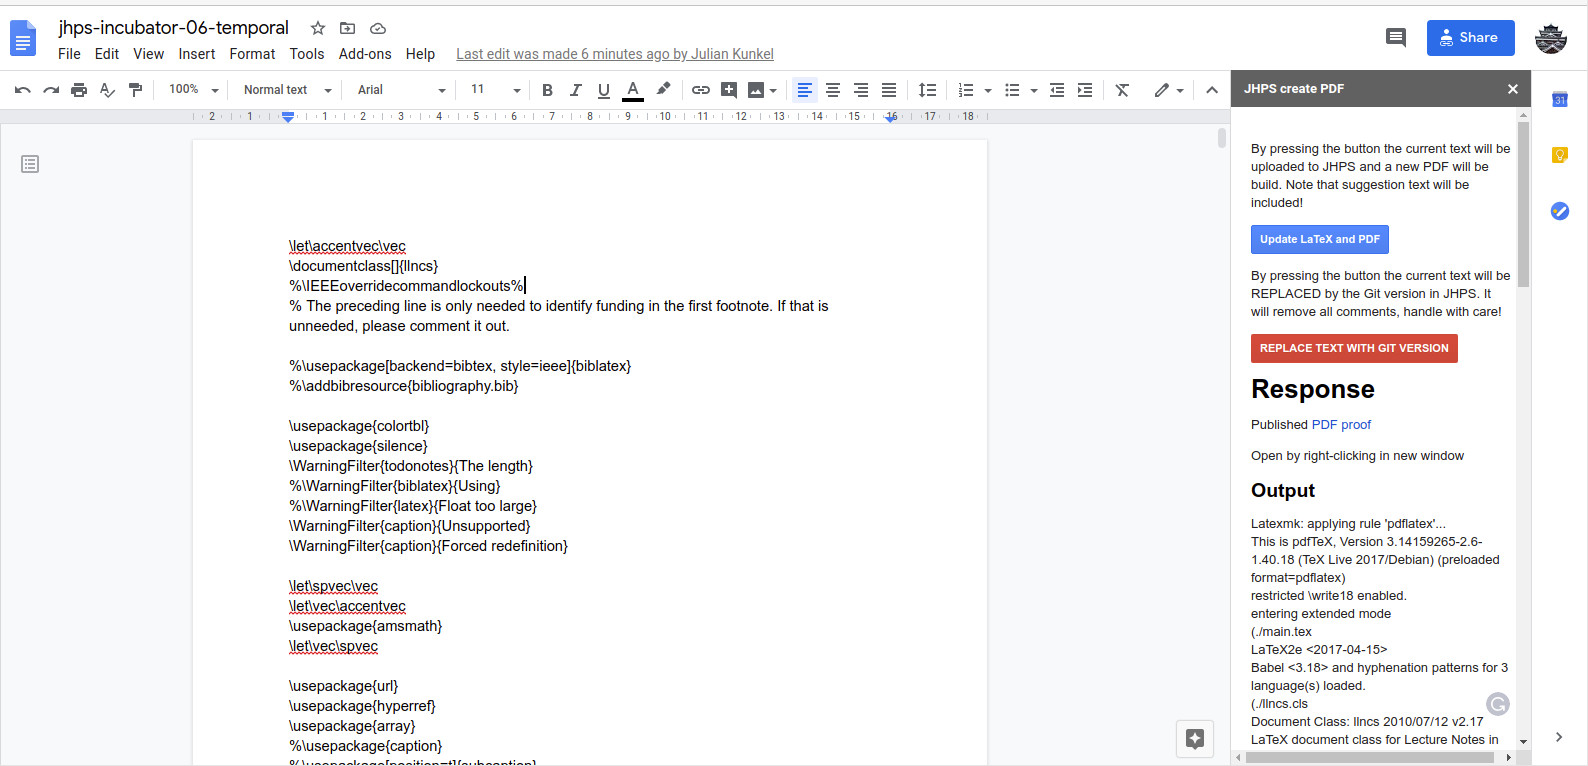
\includegraphics[width=\textwidth]{jhps}
  \caption{Caption 2}\label{fig:1b}
  \end{subfigure}
  \caption{Caption of the main figure}\label{fig:1}
\end{figure}


\subsubsection{Listings}

Use the lstlisting package for short inline listings here (ca.
5 lines) as in \Cref{lst:listing}.
Otherwise wrap it into the lstfloat environment as in \Cref{lst:longlisting}.

\begin{lstlisting}[caption="My listing",label=lst:listing,language=C,inputencoding={utf8},extendedchars=false]
int main(){
  int jhps = 1;
  printf("This article is in JHPS:   %d\n", jhps);
}
\end{lstlisting}

\begin{lstfloat}
  \begin{lstlisting}[caption="My longer listing",label=lst:longlisting,language=C]
int main(){
  // Comment
  /* comment */
  int jhps = 1;
  printf("This article is in JHPS:   %d\n", jhps);
}
  \end{lstlisting}
\end{lstfloat}


\subsection{Footnote}
Add\footnote{footnotes}.

\subsection{Links}
Generally, avoid using links in the text, but rather use a footnote, e.g.,
The webpage of JHPS\footnote{\url{https://jhps.vi4io.org}} provides author instructions.
You may also embed long links using HREF \href{https://jhps.vi4io.org}{JHPS Webpage}.

\subsection{Verbatim}
To create a verbatim environment, you can use:
\begin{verbatim}
\verb|Some verbatim text|
\end{verbatim}
or
\begin{verbatim}
\begin{verbatim}
Some verbatim text
\end{verbatim}
\vspace*{-0.8em}
\verb|\end{verbatim}|

\subsection{References}

Use the Cref command, e.g. \verb|\Cref{lst:listing}|.\subsection{Citations}

Please use the default style; example: \cite{misc1998}.
Please save the bibliography in the file \texttt{bibliography.bib}.

Generally, avoid using links in the bibliography, use a footnote instead.
Online references such as webpage, posters or presentations can be used and cited such as: \cite{link20pres, link20post, link20web}.
For the date/year, depending on the resource use the date the poster was created, the date the presentation was held (or as stored in the document, such as PDF creation date).

If you refer to a link repeatedly, you may use a citation, use as date/year the time the particular page was changed the last time (if provided, otherwise leave empty).
As author, you should use the author of the article or leave it empty otherwise.

This should be listed as in the bibliography, see \Cref{lst:bib}.
\begin{lstfloat}
\lstinputlisting[caption="The bibliography.bib file",label="lst:bib",inputencoding={utf8},language=bibtex]{bibliography.bib}
\end{lstfloat}

\subsection*{Acknowledgment} %% Remove this section if not needed
\textit{We thank XX for sponsoring.}

  % The bibliography
\addcontentsline{toc}{section}{Bibliography}
\bibliography{bibliography.bib}

\reviews   % The review section

\subsection*{Reviewer: \href{Optional URL to reviewer page}{Firstname LastName}, Date: 2020-07-07}

\paragraph{Overall summary and proposal for acceptance}

\paragraph{Scope}   % in regards to the journal, i.e., does the topic fit?

\paragraph{Significance}   % of the research, minor vs. major

\paragraph{Readability}   % English and structure appropriate?

\paragraph{Presentation}

\paragraph{References}   % Correctly formatted?

\paragraph{Correctness}   % Is the research correct


\end{document}
